\documentclass{article}

\usepackage[pdftex]{graphicx}
%\usepackage{cite}
\usepackage{indentfirst}
\setlength{\parindent}{1em}

\title{Lyapunov based Nonlinear Control - Assignment1}
\author{Sun Qinxuan}

\begin{document}
\maketitle
%\title{Lyapunov based Nonlinear Control, Assignment1}
%\author{Sun Qinxuan}

\section{Problem}

\indent simulate the following system
$$
\ddot{x}+0.1\dot{x}+x^5=6\sin{t}
$$
for two set of initial conditions
$$
x_0=2, \dot{x}_0=3
$$
and
$$
x_0=2.01, \dot{x}_0=3.01
$$

\section{Solution}

\indent Note that the given two initial conditions are almost identical.

\indent As shown in Figure \ref{response_20} and Figure \ref{phase_plane_20}, the responses of the system to the two initial conditions nearly coincide within a certain period of time (about 25s). But after that, the responses become apparently different from each other, as shown in Figure \ref{response_50} and Figure \ref{phase_plane_50}.

\indent It is due to chaos in the system caused by the high nonlinearity in $x_5$.

\begin{figure}
  \centering
  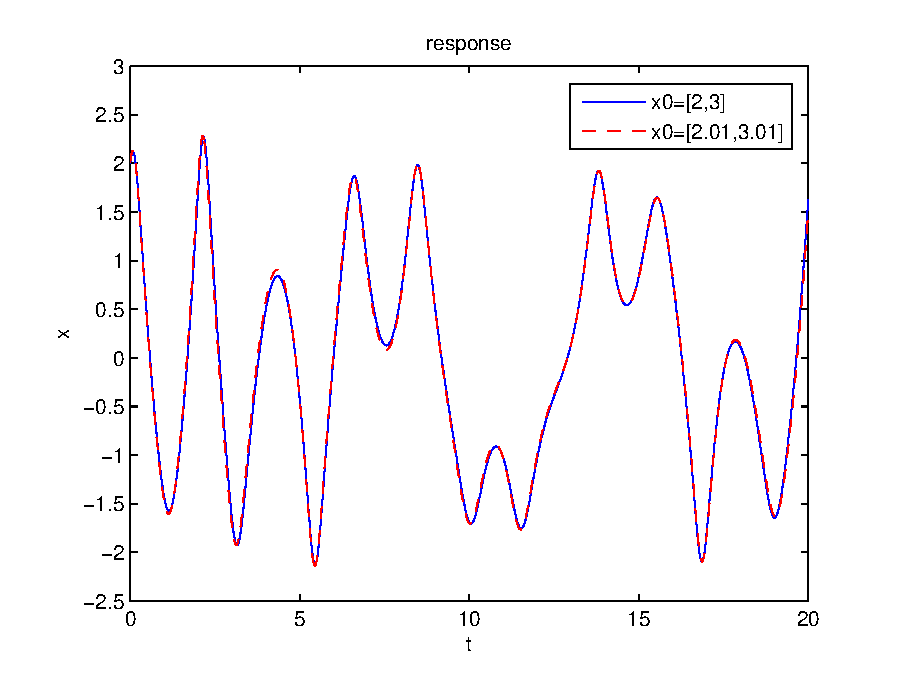
\includegraphics[width=0.8\textwidth]{figs/response_20.eps}% 1\linewidth
  \caption{the response when system runtime is 20s.}
  \label{response_20}
\end{figure}

\begin{figure}
  \centering
  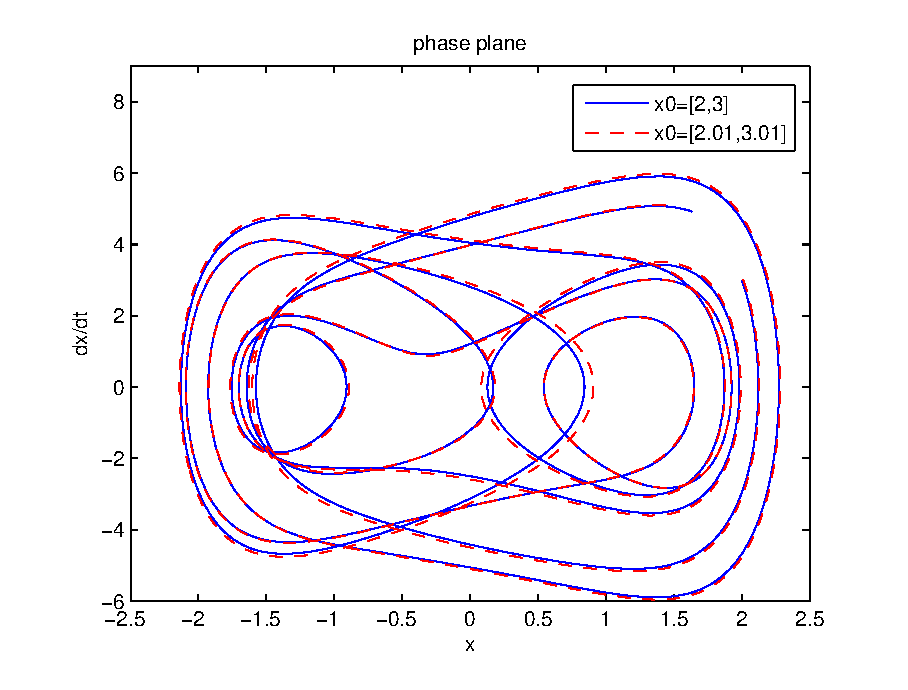
\includegraphics[width=0.8\textwidth]{figs/phase_plane_20.eps}% 1\linewidth
  \caption{the phase plane when system runtime is 20s.}
  \label{phase_plane_20}
\end{figure}

\begin{figure}
  \centering
  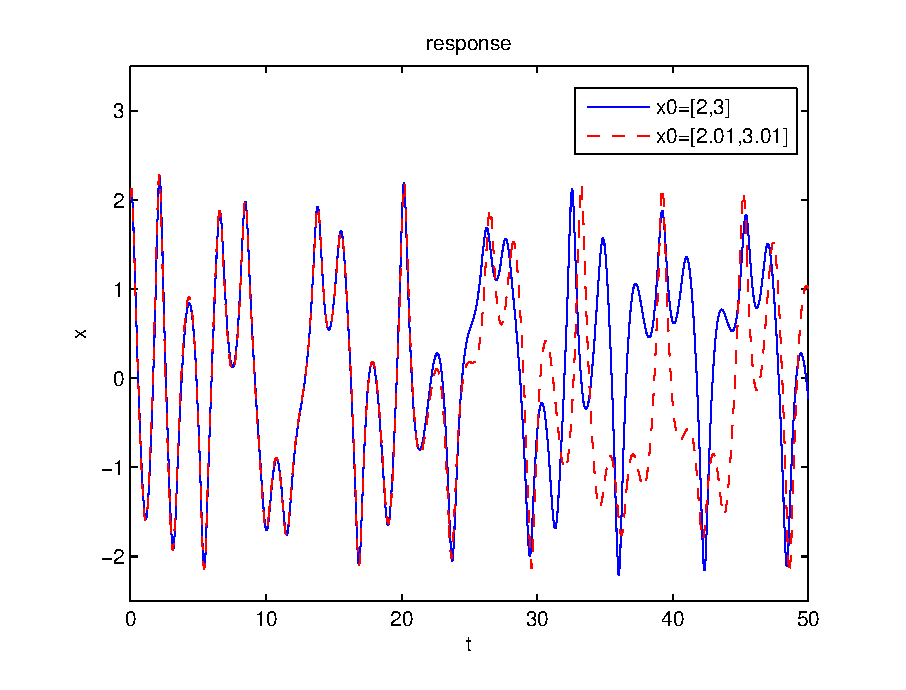
\includegraphics[width=0.8\textwidth]{figs/response_50.eps}% 1\linewidth
  \caption{the response when system runtime is 50s.}
  \label{response_50}
\end{figure}

\begin{figure}
  \centering
  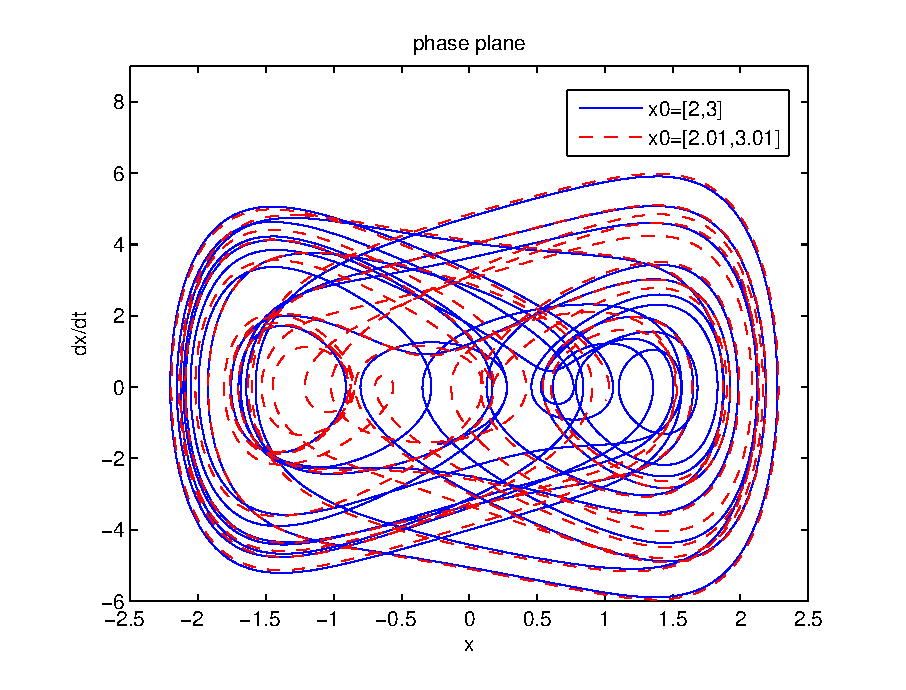
\includegraphics[width=0.8\textwidth]{figs/phase_plane_50.eps}% 1\linewidth
  \caption{the phase plane when system runtime is 50s.}
  \label{phase_plane_50}
\end{figure}

\end{document} 